\documentclass[12pt,a4paper]{report}
\usepackage[utf8]{inputenc}
\usepackage{hyperref}
\usepackage{geometry}
\usepackage{graphicx}
\geometry{a4paper, margin=1in}

\title{lorem ipsum \\ \large MIRPR Stable Diffusion Project}
\author{Eduard-Mitrut Rosca, Albert Regus}

\begin{document}

\maketitle

\chapter*{Demo APP Functionalities \& Features}

\section*{Overview}
The application is a website featuring a canvas (similar to the one provided by \href{https://www.nvidia.com/en-us/studio/canvas/}{NVIDIA Canvas}), where users can paint simple images. The output is a realistic image generated based on the user’s preferences using a Stable Diffusion-based model.

\section*{Functionalities}
\begin{itemize}
    \item Paint on a blank canvas using different brush colors and sizes.
    \item Erase unwanted elements from the canvas.
    \item Display the generated realistic image output to the user.
\end{itemize}

\section*{Short Description}
The system leverages a Stable Diffusion-based model, such as ControlNet, to generate realistic synthetic images. This approach aims to improve the performance of AI models that require large datasets to achieve optimal results by providing an efficient way to generate training data.

\chapter*{Useful Work and Related Work}

\section*{ControlNet}
ControlNet extends pretrained diffusion models by adding structural control mechanisms, enabling precise alignment of image generation with edge maps, segmentation maps, or other spatial guides.
\begin{itemize}
    \item \href{https://github.com/lllyasviel/ControlNet}{https://github.com/lllyasviel/ControlNet}
    \item \href{https://arxiv.org/pdf/2302.05543}{https://arxiv.org/pdf/2302.05543}
\end{itemize}

\section*{UNet (Used for Segmentation)}
UNet is a convolutional neural network designed for image segmentation, featuring an encoder-decoder structure with skip connections to preserve spatial information and generate precise segmentations.
\begin{itemize}
    \item \href{https://arxiv.org/pdf/1505.04597}{https://arxiv.org/pdf/1505.04597}
\end{itemize}

\section*{Fréchet Inception Distance (For Metrics)}
Fréchet Inception Distance (FID) is a metric used to evaluate the quality of generated images by measuring the similarity between feature distributions of real and generated images.
\begin{itemize}
    \item \href{https://arxiv.org/pdf/1706.08500}{https://arxiv.org/pdf/1706.08500}
\end{itemize}

\section*{Datasets}
Publicly available datasets used for training and evaluating generative models, particularly in tasks involving depth estimation, segmentation, and indoor scenes.
\begin{itemize}
    \item \href{https://cs.nyu.edu/~fergus/datasets/nyu_depth_v2.html}{NYU Depth Dataset V2}
    \item \href{https://cs.nyu.edu/~fergus/datasets/indoor_seg_support.pdf}{Indoor Segmentation Support (ADE20K)}
\end{itemize}

\section*{Generative Models (StabilityAI)}
StabilityAI provides state-of-the-art generative models, including open-source tools and pretrained resources, for creating high-quality synthetic images.
\begin{itemize}
    \item \href{https://github.com/stability-ai/generative-models}{https://github.com/stability-ai/generative-models}
\end{itemize}

\section*{Stable Diffusion}
Stable Diffusion is a diffusion-based generative model capable of creating high-quality images from textual prompts, leveraging large-scale training for versatility and precision.
\begin{itemize}
    \item \href{https://arxiv.org/pdf/2112.10752}{https://arxiv.org/pdf/2112.10752}
\end{itemize}



\chapter*{Training on ToyDataset}

\section*{ControlNet}
ControlNet is a pretrained diffusion model used in image generation tasks, particularly for applications that require precise control over generated outputs based on user inputs. By using control structures like edge maps or human pose estimations, ControlNet allows users to guide the diffusion process for targeted and customizable image synthesis. This feature makes it highly suitable for real-world applications where the image content needs to closely match specified criteria, making it particularly useful in tools that require user-driven adjustments to generated images.
\begin{itemize}
    \item \href{https://github.com/lllyasviel/ControlNet}{ControlNet GitHub Repository}
    \item \href{https://arxiv.org/pdf/2302.05543}{ControlNet Research Paper}
\end{itemize}

How it works

    

\subsection*{Fill50k DataSet}

The Fill50k dataset used in this project is specifically designed to support training in image generation tasks involving circular shapes.

- Source Images with Circle Masks: The dataset contains source images that include masks of circles. These masks serve as structural guides for models, helping them learn the spatial arrangement and shape of circles within an image. By providing masked regions, these source images establish the foundational patterns that guide the model in generating circular forms.

- Target Images for Training: In addition to source images with masks, Fill50k includes target images, which are the desired outputs the model aims to replicate or generate. These target images allow the model to learn the texture, color, and lighting details that should fill the circular masked areas, effectively helping it understand how to realistically render circles.

- Text Prompts: Each image in the Fill50k dataset is associated with a specific prompt used during training. These prompts describe the image content, helping the model learn to associate textual descriptions with visual features.

\subsection*{How We Used ControlNet}
In our project, we trained the ControlNet model to generate circular images by training it for 3 and 5 epochs on a dataset of 512 images from the Fill50k dataset. This customization allows the model to produce outputs tailored to our specific requirements for generating circle images on the application’s canvas.
We used the Stable Diffusion 2.1 (SD2.1) model for training. However, since the training was performed on a limited dataset of only 512 images, we encountered some inconsistencies in the generated images. Specifically, although the model was trained to generate circular images based on a prompt, the textures in the background of the generated images did not always match those found in the training data (example: Figure2). This issue arose because the limited size and diversity of the training dataset resulted in insufficient generalization of background textures for the same prompts. Despite this, the model was able to capture the core features, such as shapes and structures, while the textures varied depending on the context of the input.
For preprocessing, images were resized to a fixed resolution of 512x512 pixels for consistent training. Also, uniformer detection was applied to generate structural maps for the source images.  The batch size used was small (between 4 and 8) because of the high computational costs. 

\begin{figure}
    \centering
    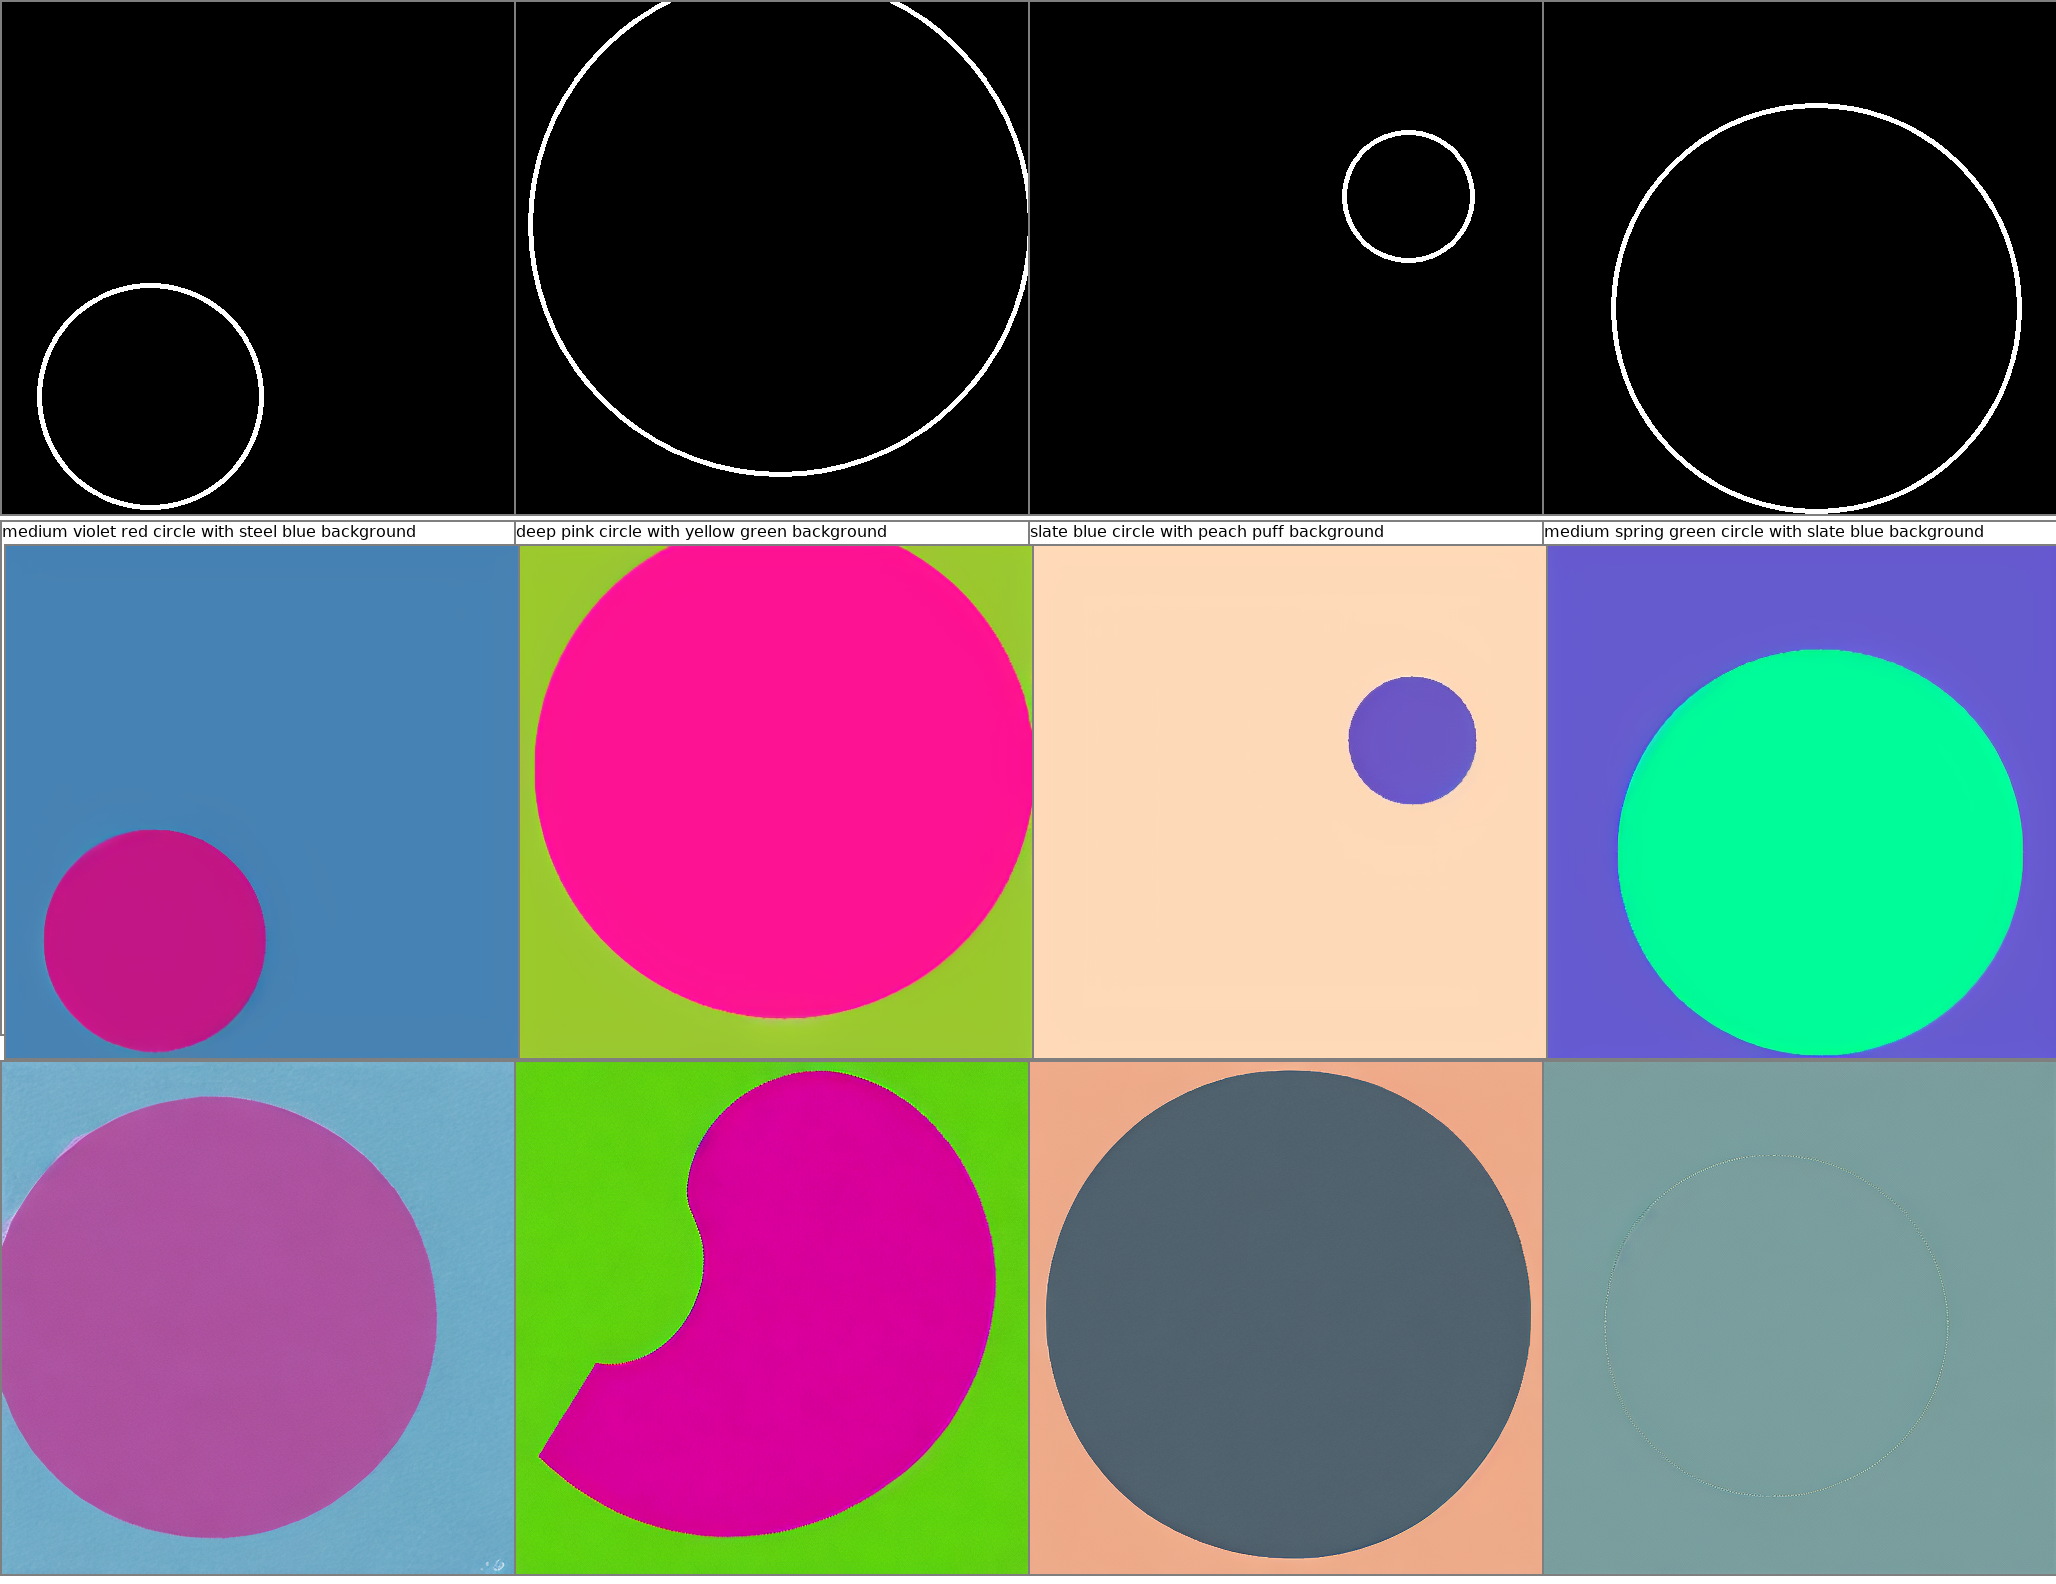
\includegraphics[width=1\linewidth]{t1e0.png}
    \caption{Example1}
    First row is the segmentation mask that is needed for structural guidance. Second row represents the target images and the last row represents the generated images by the model using the mask and the prompt.
\end{figure}

\begin{figure}
    \centering
    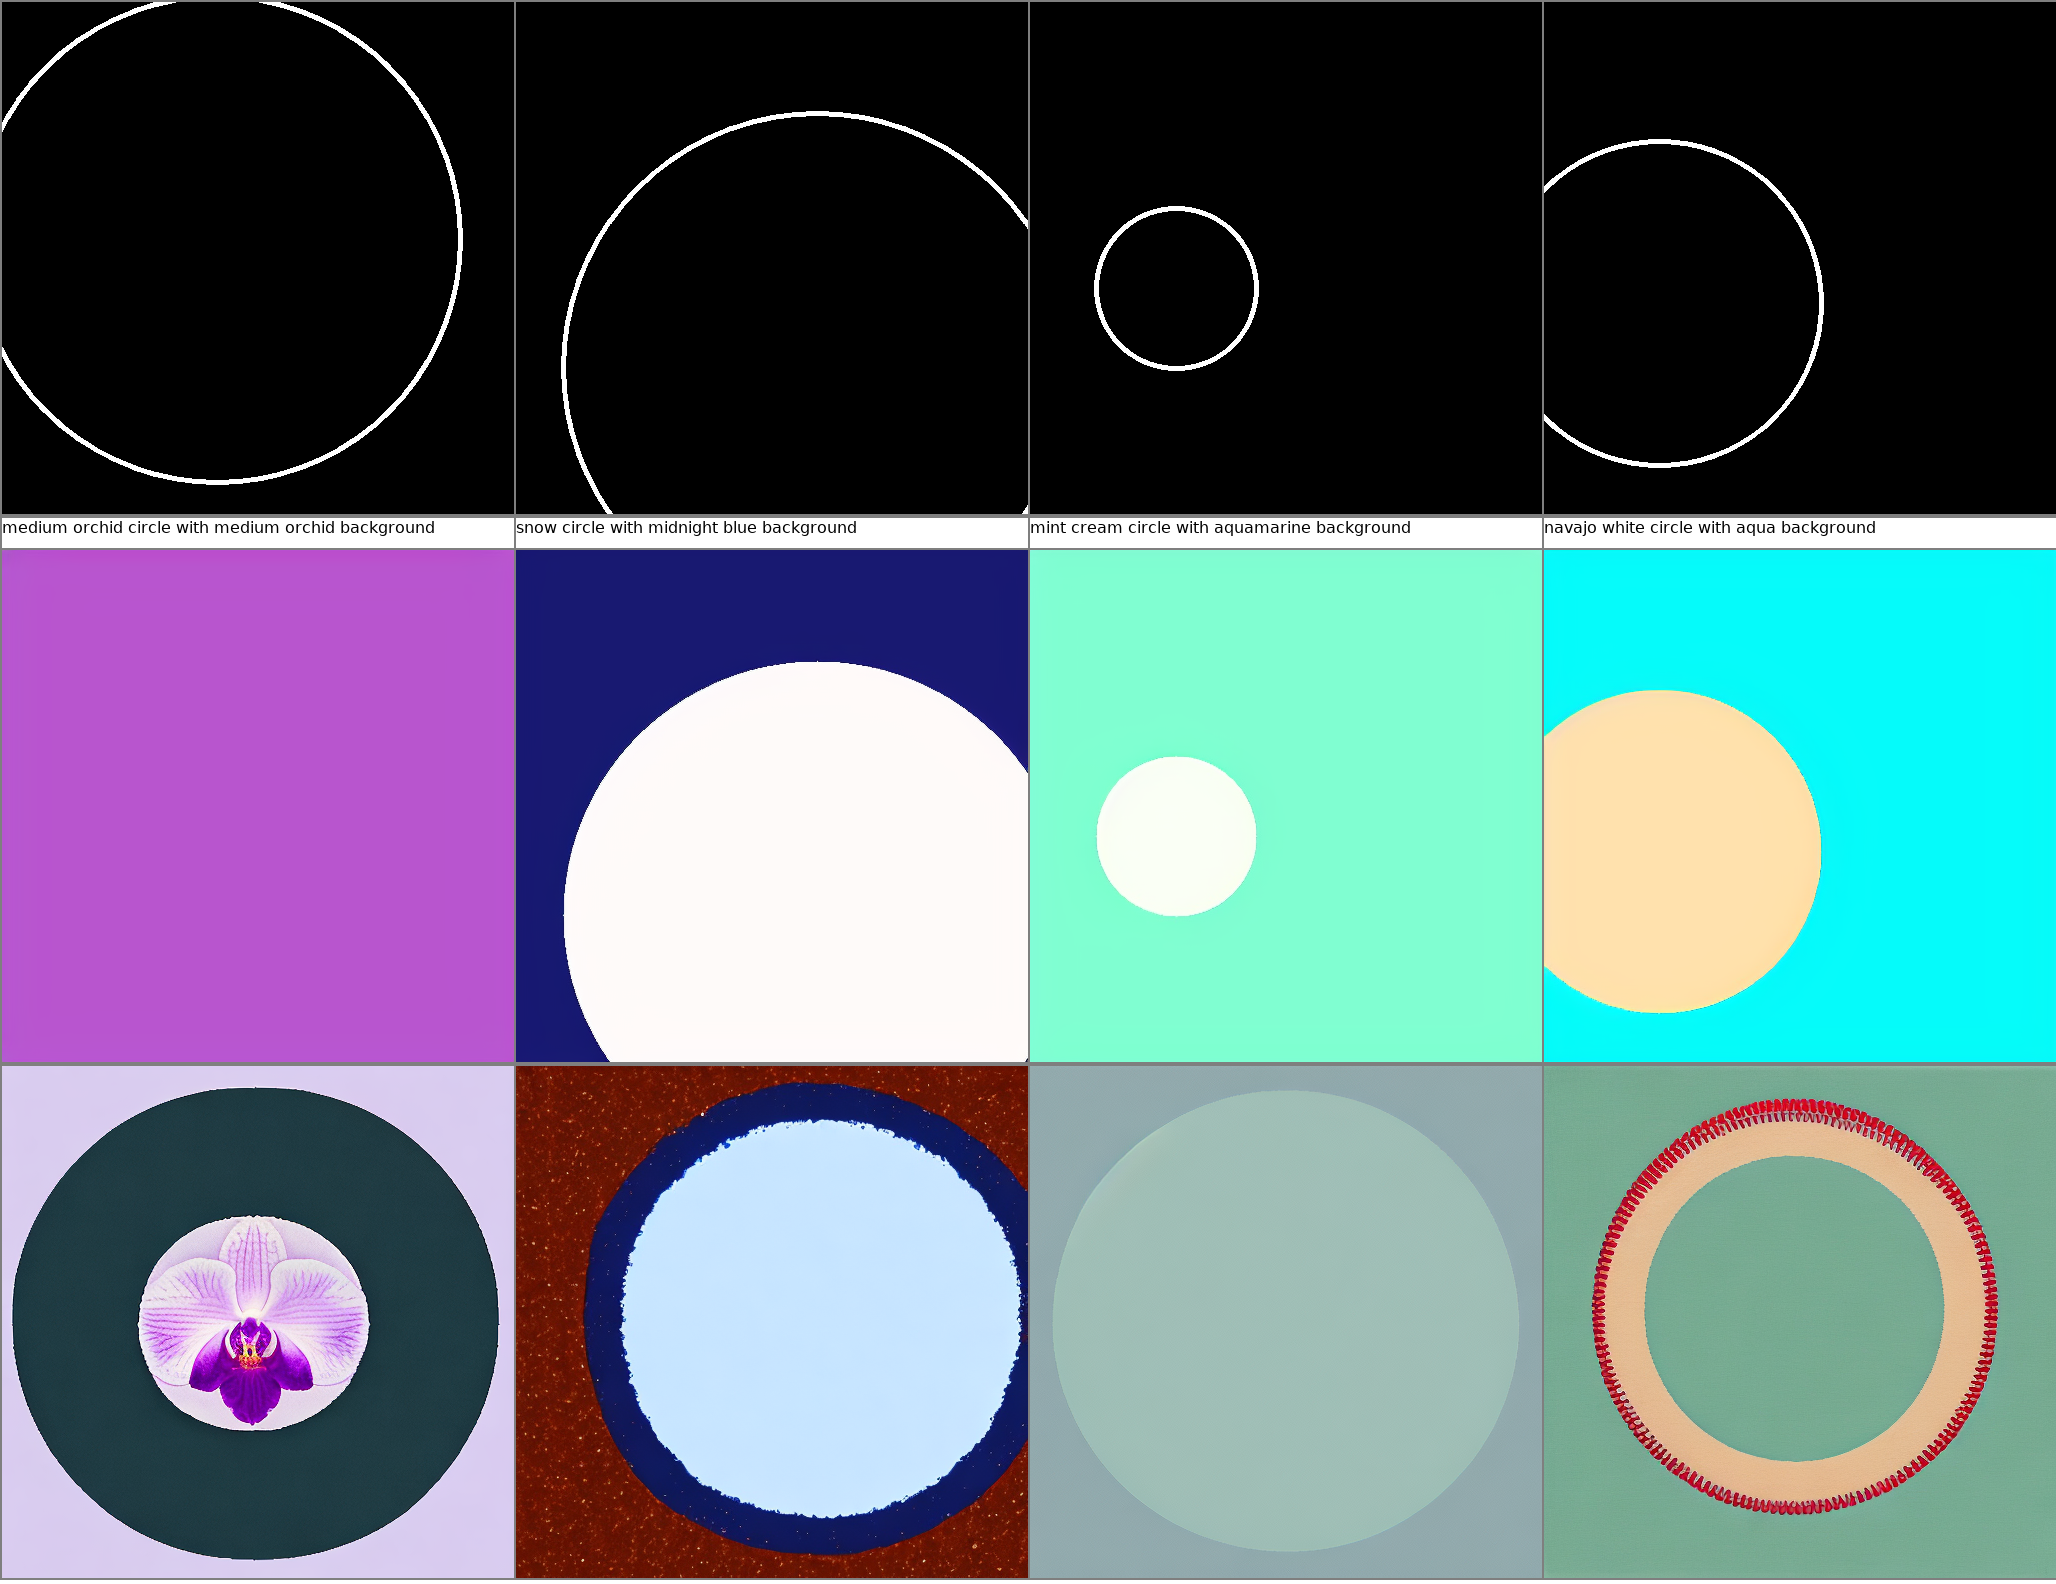
\includegraphics[width=1\linewidth]{t1e2.png}
    \caption{Example2}
        First row is the segmentation mask that is needed for structural guidance. Second row represents the target images and the last row represents the generated images by the model using the mask and the prompt.
\end{figure}

\subsection*{Challenges in Model Training and Final Solution Using LightningAI}

We encountered some challenges during the process of training a machine learning model due to limited resources and issues with various platforms. Initial attempts to train the model locally were hindered by insufficient resources. Subsequently, we experimented with training on \href{https://colab.research.google.com/}{Google Colab}, but encountered memory constraints due to inadequate RAM. Attempts to use \href{https://www.kaggle.com/}{Kaggle} were met with configuration issues related to the Anaconda environment. Ultimately, we achieved successful model training on \href{https://lightning.ai/}{LightningAI}, which provided a stable and resourceful platform for completing our training.

\subsection*{Evolution of the loss function and the quality of the generated images}

\title{SSIM (Structural Similarity Index Measure)}

To calculate the similarity between the ground truth and the generated images we used SSIM (Structural Similarity Index Measure). This metric measures the similarity between two images by considering changes in the structural information, luminance and contrast. It works by comparing local patterns of pixels, searching for luminance (brightness), contrast (texture), structure (patterns). To get the luminance, the metric measures the brightness between two images. For contrast, the metric measures the similarity in contrast (intensity) and for structure the metric measures the similarity in the patterns of pixel intensities. The overall SSIM Score is the combination of those three components. A SSIM Score of 1 indicates that the images are identical, a score close to 1 indicates that the images are similar but with minor differences and a score of 0 indicates that the images are completely different.


\begin{figure}
    \centering
    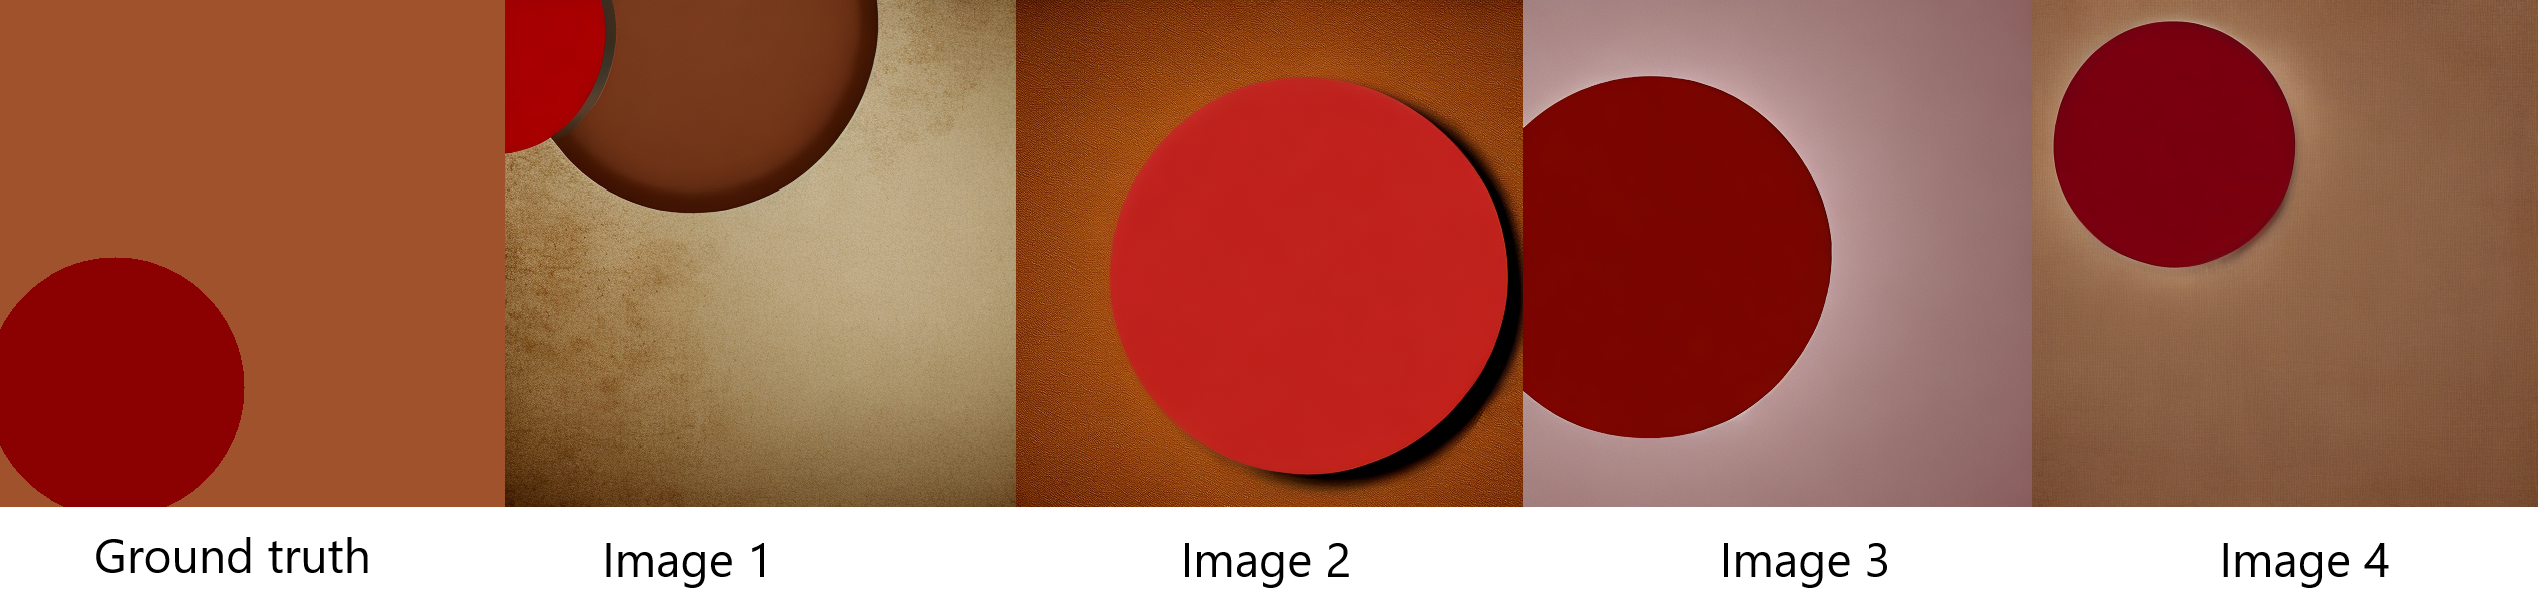
\includegraphics[width=1\linewidth]{circle_images_ssid_metric.png}
    \caption{Ground truth image and 4 images generated}
    \label{fig:enter-label}
\end{figure}

\begin{figure}
    \centering
    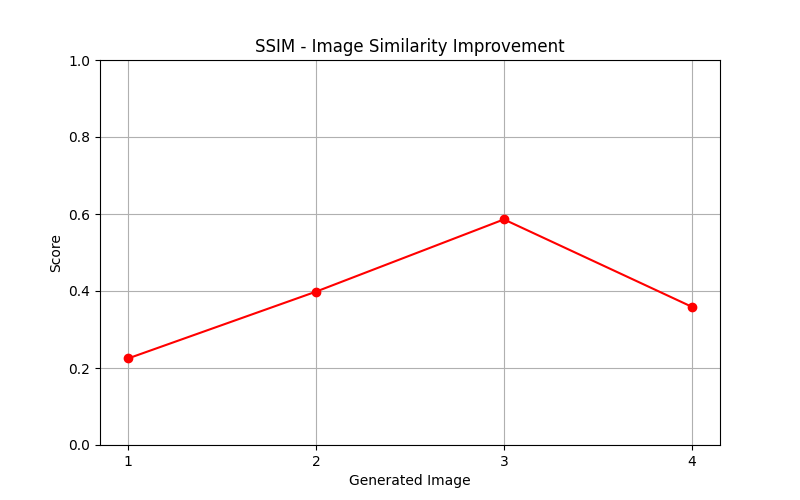
\includegraphics[width=0.75\linewidth]{similarity_improvement.png}
    \caption{SSIM Score and the rate of improvement}
    \label{fig:enter-label}
\end{figure}

We calculated the SSIM Score using the images in Figure 3. The first image has a score close to 0.2 which means the image is completely different. The score increased as the images were generated and the biggest SSIM Score was close to 0.6 which means the images have similarities but also some differences. The SSIM Score is not so high because we used a reduced dataset of 512 images because of a lack of computing performance.

\chapter*{Training on Real Dataset}

\subsection*{Dataset}

For training, we used four datasets:
\begin{itemize}
    \item \textbf{Cityscapes Dataset}: \url{https://www.cityscapes-dataset.com/}
    \item \textbf{CamVid Dataset} \url{https://paperswithcode.com/dataset/camvid}
    \item \textbf{WildDash 2}: \url{https://wilddash.cc/}
    \item \textbf{KITTI Dataset}: \url{https://www.cvlibs.net/datasets/kitti/}
\end{itemize}

To ensure consistency in file structure and resolution across all files, the CamVid and WildDash 2 datasets were modified to match the structure of the Cityscapes Dataset.

The unified dataset contains images of cityscapes and traffic images with a resolution of 1024x512 pixels and their corresponding masks.

\begin{figure}[h]
    \centering
    % First image
    \begin{minipage}{0.45\textwidth}
        \centering
        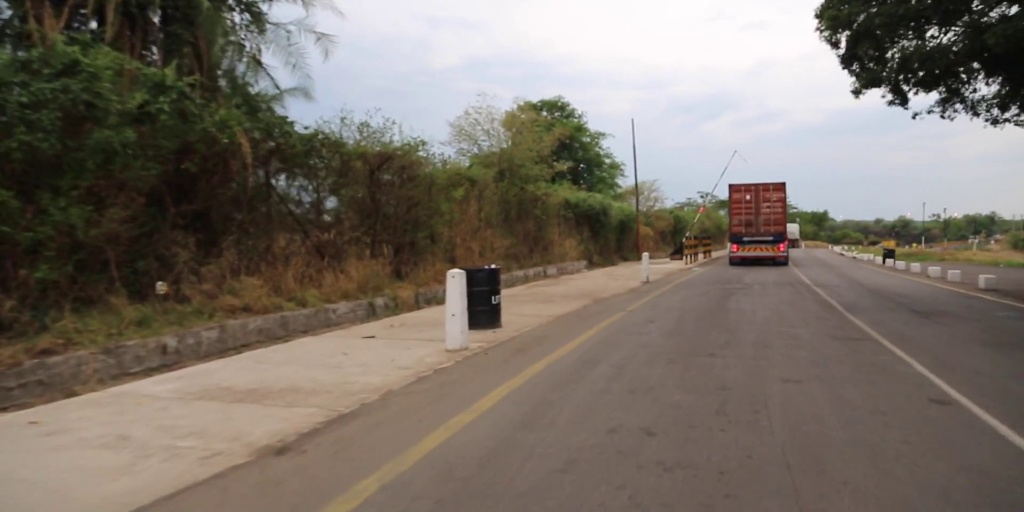
\includegraphics[width=\textwidth]{zw0000_100000.jpg}
        \caption{Original image.}
        \label{fig:image1}
    \end{minipage}
    \hfill
    % Second image
    \begin{minipage}{0.45\textwidth}
        \centering
        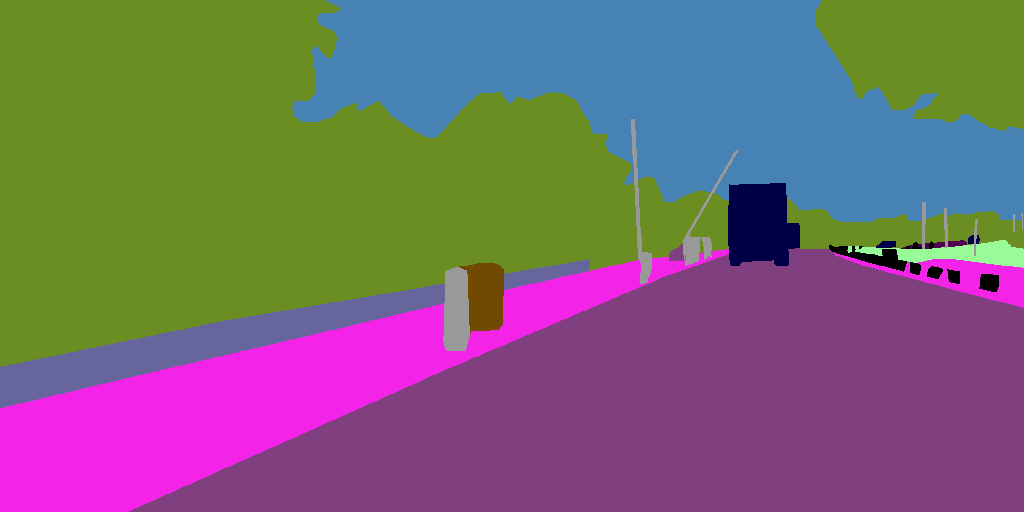
\includegraphics[width=\textwidth]{zw0000_100000_labelIds.png}
        \caption{Segmentation mask of the corresponding image.}
        \label{fig:image2}
    \end{minipage}
    \caption{Example of an image from dataset}
    \label{fig:combined_images}
\end{figure}

\subsection*{Training}

\subsection*{Training Overview}

The training process involves fine-tuning a pre-trained model, specifically the \href {https://huggingface.co/lllyasviel/ControlNet/blob/main/models/control_sd15_seg.pth} {Control SD 15}, to adapt it to a custom dataset. The model used in this process is based on a version of the Stable Diffusion model, which has been pre-trained on a large dataset and then further trained on our data.

The training runs for 2 epochs, where each epoch consists of processing the entire dataset once. This allows the model to process the data in smaller, manageable parts, improving efficiency and performance. The model is trained with a learning rate of 1e-5, a parameter that controls the speed at which the model adjusts during each training step.

Throughout the training, the model’s performance is tracked using loggers. Images generated by the model are saved regularly to monitor its progress, while metrics such as the loss function are also recorded to evaluate how well the model is learning.

To ensure that training progress is not lost, the model's weights are saved at regular intervals. At the end of the training, the final version of the model is saved, allowing it to be used later for generating results or further fine-tuning.

In summary, the training involves fine-tuning a pre-trained Control SD15 Segmentation model on a custom dataset for 2 epochs, using batches of 2 images, while tracking progress and saving the model at the end of the process.

\begin{figure}[h]
    \centering
    % First image
    \begin{minipage}{1\textwidth}
        \centering
        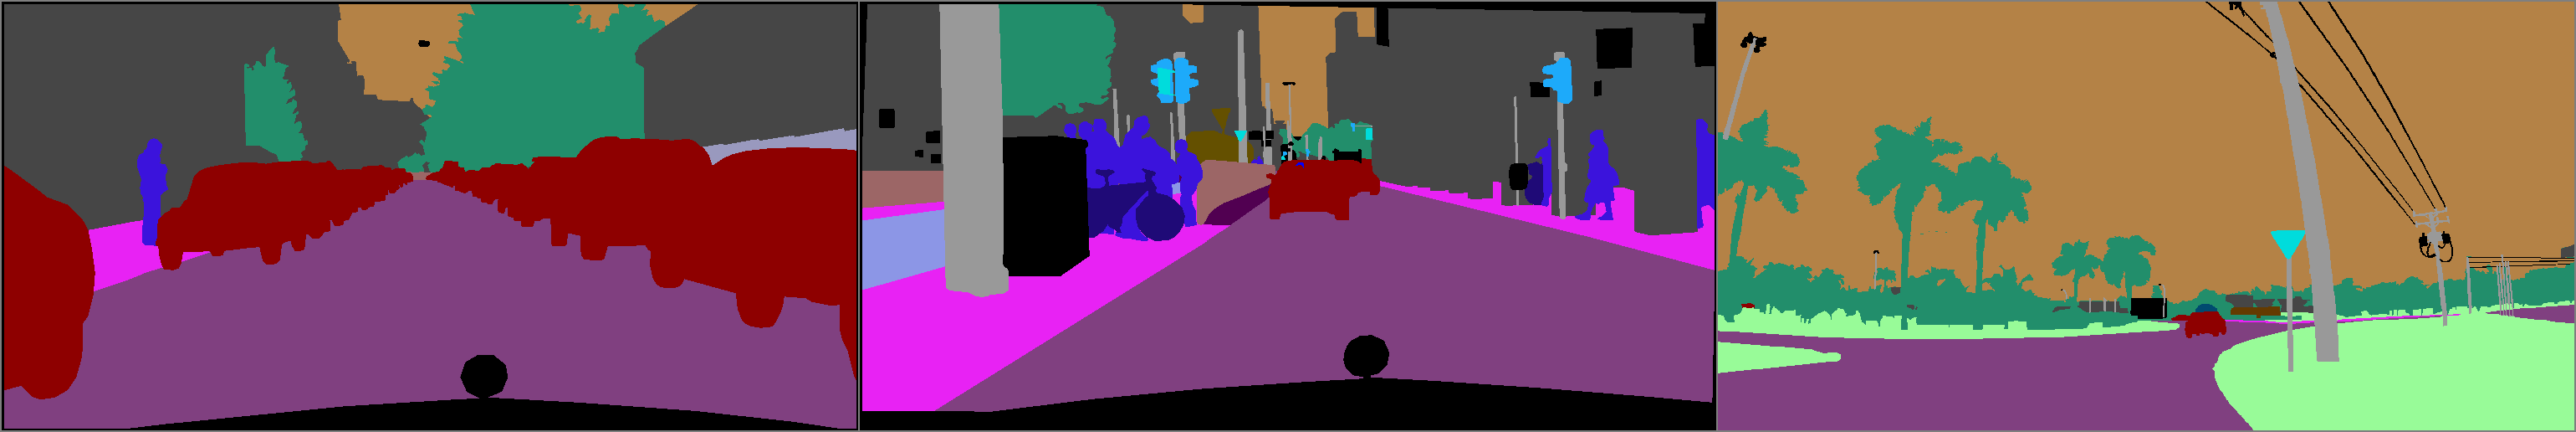
\includegraphics[width=\textwidth]{control_gs-003500_e-000001_b-001500.png}
        \caption{Segmentation mask}
        \label{fig:image1}
    \end{minipage}
    \hfill
    % Second image
    \begin{minipage}{1\textwidth}
        \centering
        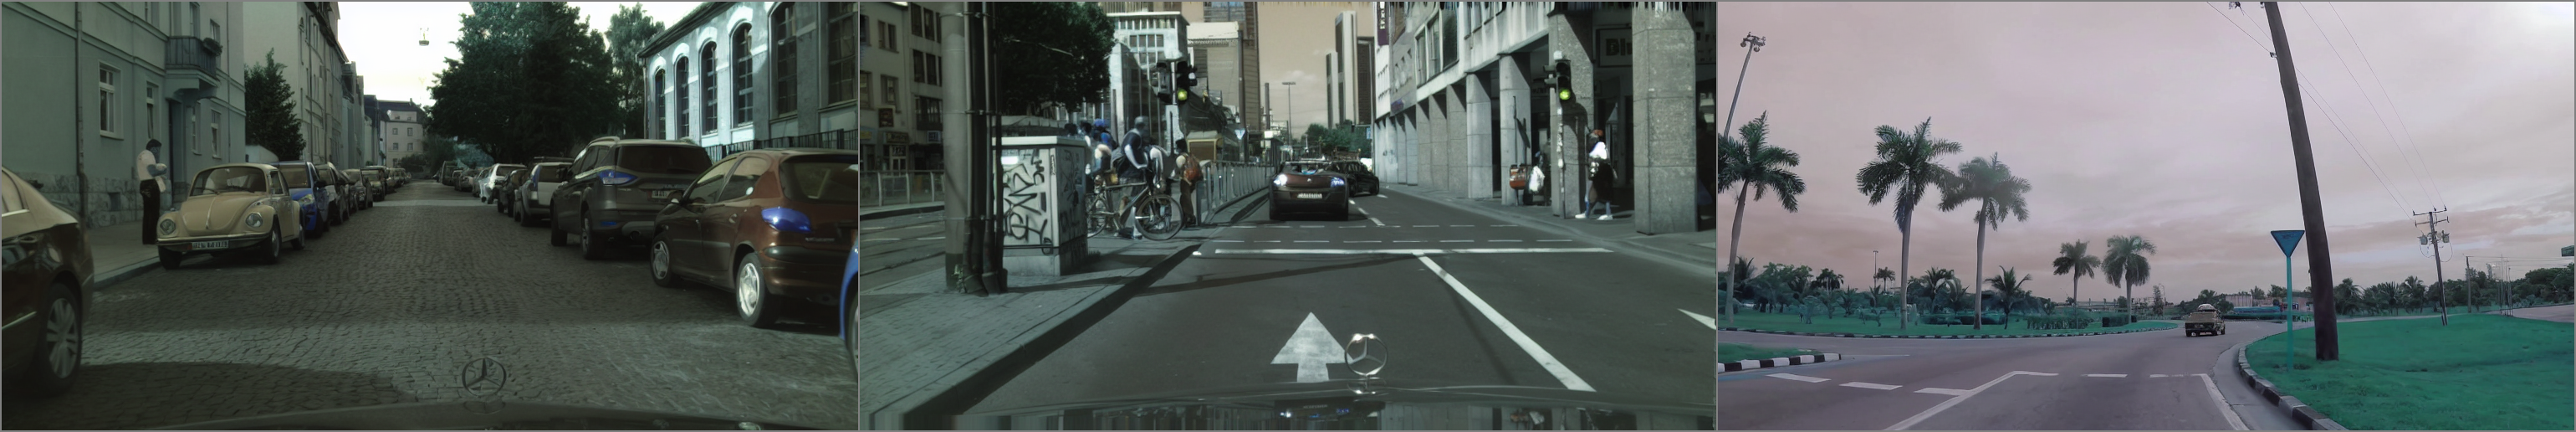
\includegraphics[width=\textwidth]{reconstruction_gs-003500_e-000001_b-001500.png}
        \caption{Original image.}
        \label{fig:image2}
    \end{minipage}
    % Third image
        \begin{minipage}{1\textwidth}
        \centering
        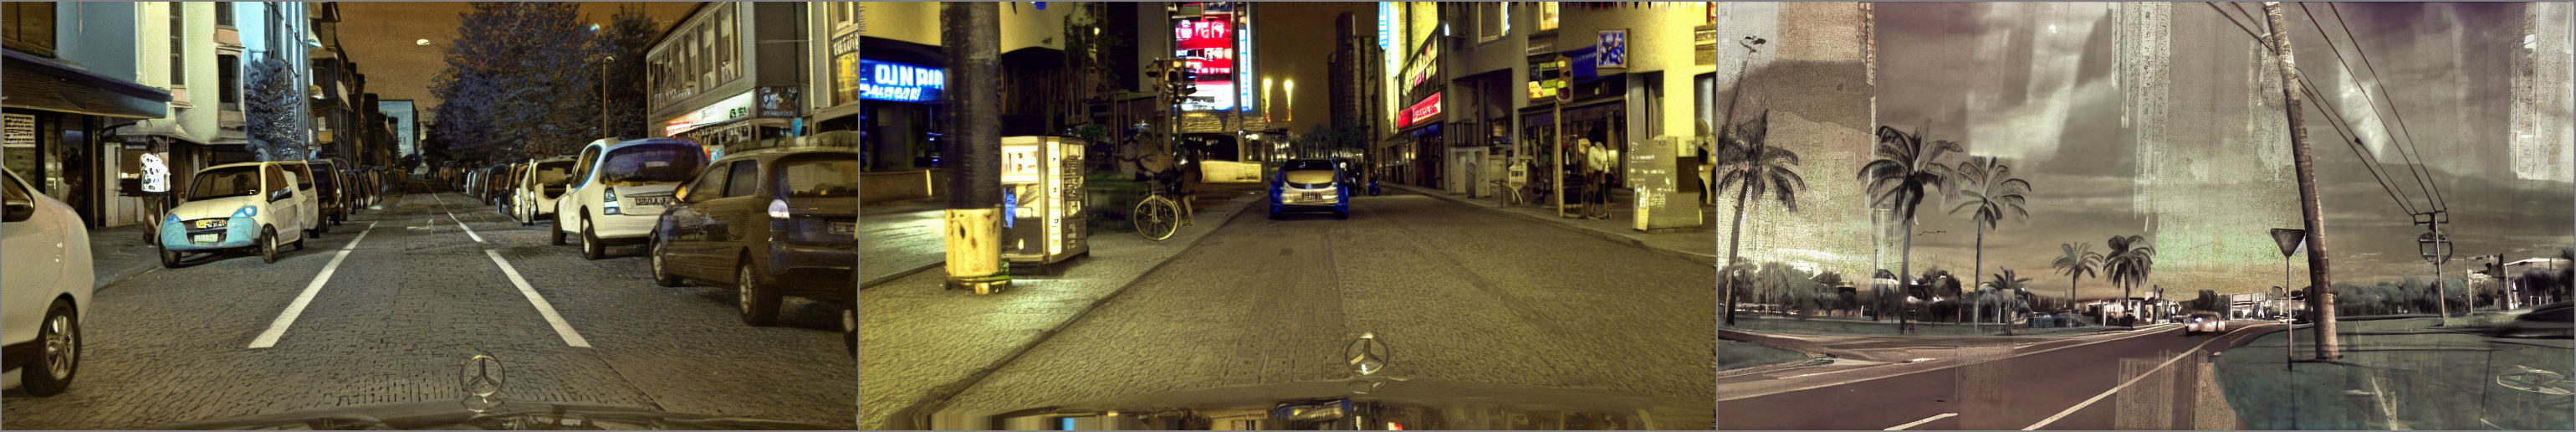
\includegraphics[width=\textwidth]{samples_cfg_scale_9.00_gs-003500_e-000001_b-001500.png}
        \caption{Generated image.}
        \label{fig:image2}
    \end{minipage}
\end{figure}


\subsection*{ Training Approaches}

For the training, we utilized different approaches to the input:

\subsection*{1. Training Using Segmentation Masks as Input}
The model was trained using only the segmentation mask as input, which provides information about the regions of specific objects, such as cars, buildings, and people. The segmentation mask-based model utilized 583.269.568 parameters and required approximately 39 seconds for inference.

\subsection*{2. Training Using Depth Masks as Input}
In this case, the model was trained using only the depth map as input. The depth map offers a representation of the distance of objects from the viewpoint, reflecting their geometric and depth-related properties. This depth map-based model utilized 583.258.048 parameters and had an inference time of about 31 seconds.

\subsection*{3. Training Using Both Segmentation Masks and Depth Masks}
The model was also trained using both segmentation masks and depth maps. This combined approach merged spatial information with depth data, offering a more comprehensive representation. It was found to be the most efficient method, with the generated output closely aligning with the target. This combined model required 583.275.328 parameters and had an inference time of around 32 seconds.

\begin{figure}[h]
    \centering
    % First image
    \begin{minipage}{0.6\textwidth}
        \centering
        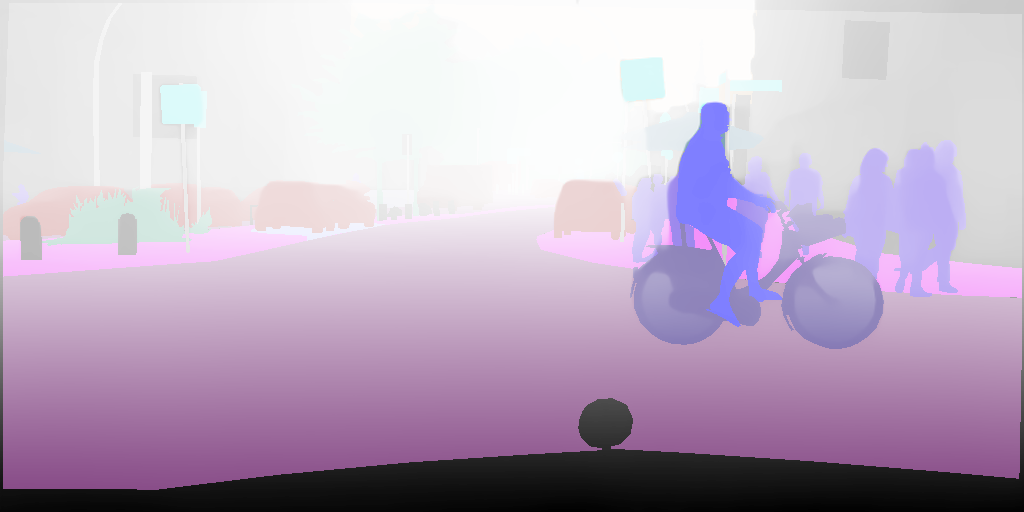
\includegraphics[width=\textwidth]{17_before_output.png}
        \caption{Segmentation mask combined with the Depth mask}
        \label{fig:image1}
    \end{minipage}
    \hfill
    % Second image
    \begin{minipage}{0.6\textwidth}
        \centering
        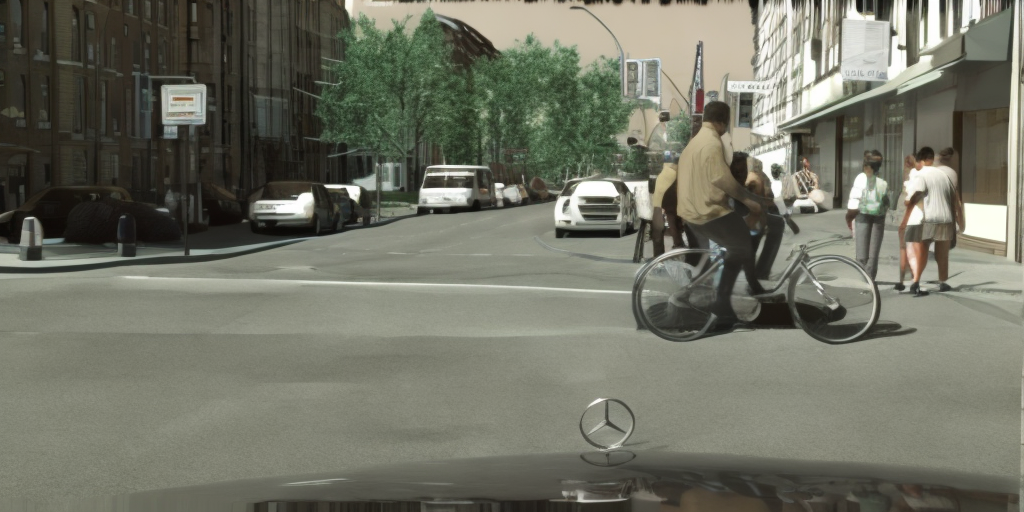
\includegraphics[width=\textwidth]{17_output.png}
        \caption{Generated image.}
        \label{fig:image2}
    \end{minipage}
    % Third image
        \begin{minipage}{0.6\textwidth}
        \centering
        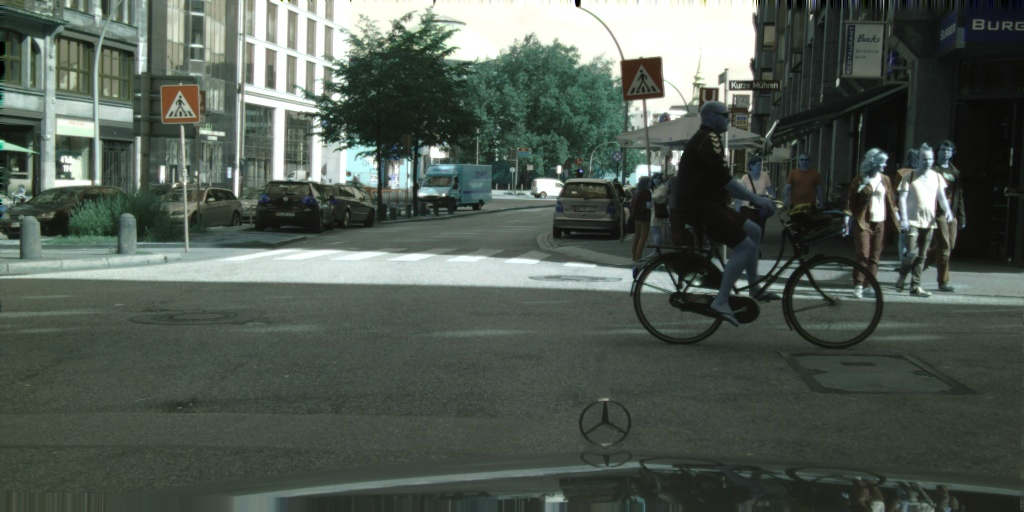
\includegraphics[width=\textwidth]{17_target.png}
        \caption{Target image.}
        \label{fig:image2}
    \end{minipage}
\end{figure}

\subsection*{ Frechet Inception Distance}

The Frechet Inception Distance (FID) is a metric used to evaluate the quality of generated images by comparing their statistical similarity to real images. It measures the difference between the distributions of real and generated images in the feature space of a pre-trained InceptionV3 network.

Lower FID scores indicate that the generated images are closer in quality and diversity to real images, with a score of 0 representing perfect similarity.

The comparison between models was done using FID to determine the model that generates the most accurate images.
Model 1 is the model that takes only the segmentation masks and the FID score was 201.37112426757812.
Model 2 is the model that takes only the depth masks and the FID score was 222.63893127441406.
Model 3 is the model that takes both the segmentation and the depth masks and the FID score was 175.92831420898438.
Also we checked the FID score for 2 different images and the score was 322.4599609375

\begin{figure}
    \centering
    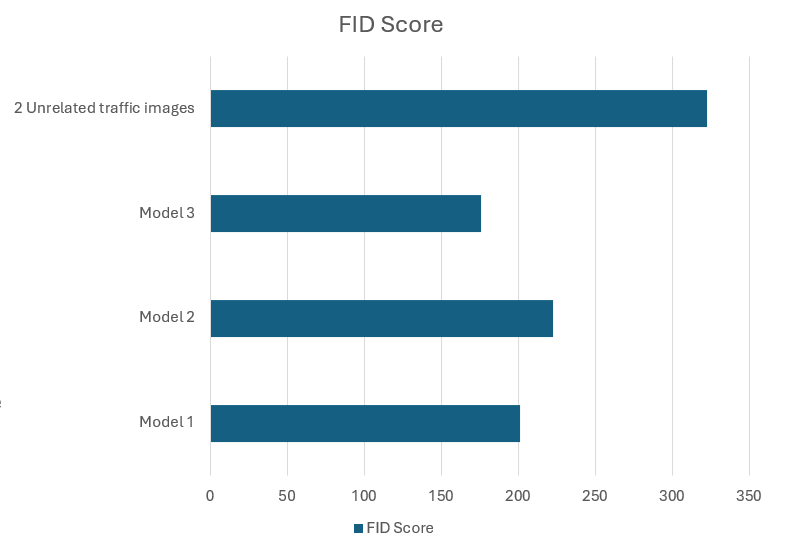
\includegraphics[width=1\linewidth]{fid.png}
    \caption{Comparison between the generated images from different models}
    \label{fig:enter-label}
\end{figure}

\subsection*{ SSIM}

The SSIM (Structural Similarity Index) score is not relevant for this set of images because the generated images have different contrast and luminosity compared to the reference images. SSIM is particularly sensitive to such differences, as it measures similarity in terms of structural, luminance, and contrast components.

% \begin{figure}
%     \centering
%     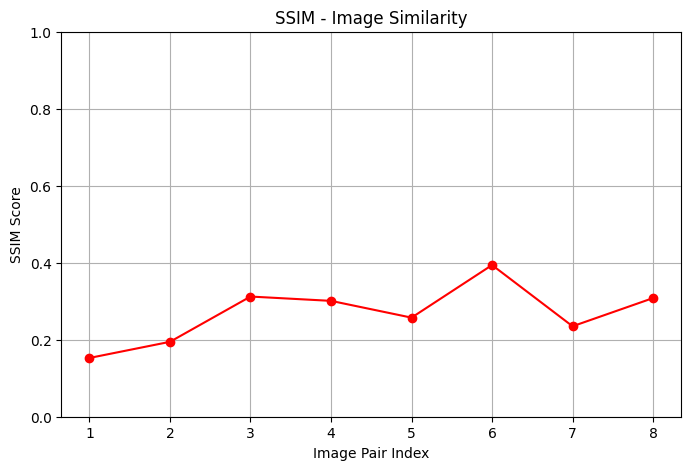
\includegraphics[width=0.5\linewidth]{1b1f40eb-5ed0-4b36-9636-1d5af3e8d98d.png}
%     \caption{SSIM Index between the original image and the generated image}
%     \label{fig:enter-label}
% \end{figure}

\end{document}